\section{Why do methodologies exist?}
\label{sec:meth_why}
A way to answer a research question in a reliable and repeatable manner is to use a systematic literature review.
According to \cite{xiao_2017}, a systematic literature review can be conducted using the following 8 steps:
\begin{enumerate}
    \item Formulate the research problem

      This involves creating the research question(s) to guide the research inquiry.
      If the question is too broad, then the data to review will be huge and unmanageable, requiring the question to be divided into sub topics.
      And getting the question right the first time maybe unlikely, in which case iterations can be used to identify the appropriate question.
    \item Develop and review the research protocol

      The review protocol is a preset plan outlining the methods used to conduct the review.
      This is done to reduce bias during data selection and analysis while at the same time increasing the repeatability of the review.
    \item Search the literature

      The literature is searched in a systematic way to answer the question identified in step 1.
      Searching involves three major sources: electronic databases; backward searching; and forward searching.
      To search electronic databases, the keywords used for the search needs to be established together with other search restrictions like publication language, data range of publications, and sources of financial support.
    \item Screen for inclusion

      The search results need to be screened to remove irrelevant results that will not contribute to the final data extraction.
      Doing a first initial screening based on the abstracts followed by an assessment of the full-text (step 5) is considered an effective procedure.
      A set of criteria for inclusion/exclusion, therefore, needs to be established to ensure the reproducibility of the review.
    \item Assess quality

      This is the final trimming down of results before data is extracted.
      Here each result is reviewed based on a full-text assessment against an established quality checklist.
      This checklist can result in the ranking of results to be used to either give the extracted data a quantative weight or by placing them qualitavely for constructing arguments.
    \item Extract data

      Depending on the type of systematic literature review, the data is extracted from the results and recorded in a format for further analysis.
    \item Analyze and synthesize data

      Here tables, charts, and textual descriptions of the data is created as needed by the type of review being conducted.
    \item Report findings

      The process used to conduct the review is reported in enough detail to be able to reproduce the study.
      The findings of the review is reported in a clear structure where the studies might be grouped into themes and characteristics.
      Novel findings and unexpected results are highlighted before the report is concluded.
\end{enumerate}

Using these 8 steps, a systematic literature review was conducted to answer the research problem for this section.

\subsection{Formulate the research problem}
The research problem for this section is finding out ``why were methodologies created''.
This will aid in understanding the types of problems methodologies try to solve and, therefore, why methodologies are still useful today.

\subsection{Develop and review the research protocol}
A descriptive systematic literature review was conducted.
This resulted in a review protocol that only considered articles, conference proceedings, and book chapters.

The search criteria was for titles to include any of the following phrases:
\begin{itemize}
    \item development methodology
    \item software development process
    \item software development lifecycle
    \item software development life cycle
\end{itemize}

While any of the following needed to appear in the abstract:
\begin{itemize}
    \item creation
    \item create
    \item purpose
    \item use
    \item benefit
\end{itemize}

The initial review protocol searched for these phrases anywhere in the article, but this resulted in more than 20,000 results.
Therefore, the requirement on the title was established to ensure articles focused on methodologies.
And the requirement on the abstract is to help tunnel articles focusing on the ``why'' aspect.

\subsection{Search the literature}
With this review protocol, the following collections were searched:

\begin{table}[H]
\begin{tabular}{ |l|r|r| }
  \hline
  Collection & Result Count & Selected \\
  \hline
  ScienceDirect & 32 & ? \\
  ACM & 55 & ? \\
  Emarald & 13 & ? \\
  ProQuest & 126 & ? \\
  EBSCOHost & 102 & ? \\
  IEEE & 243 & ? \\
  \hline
\end{tabular}
\label{table:search_lit}
\end{table}

\begin{figure}[H]
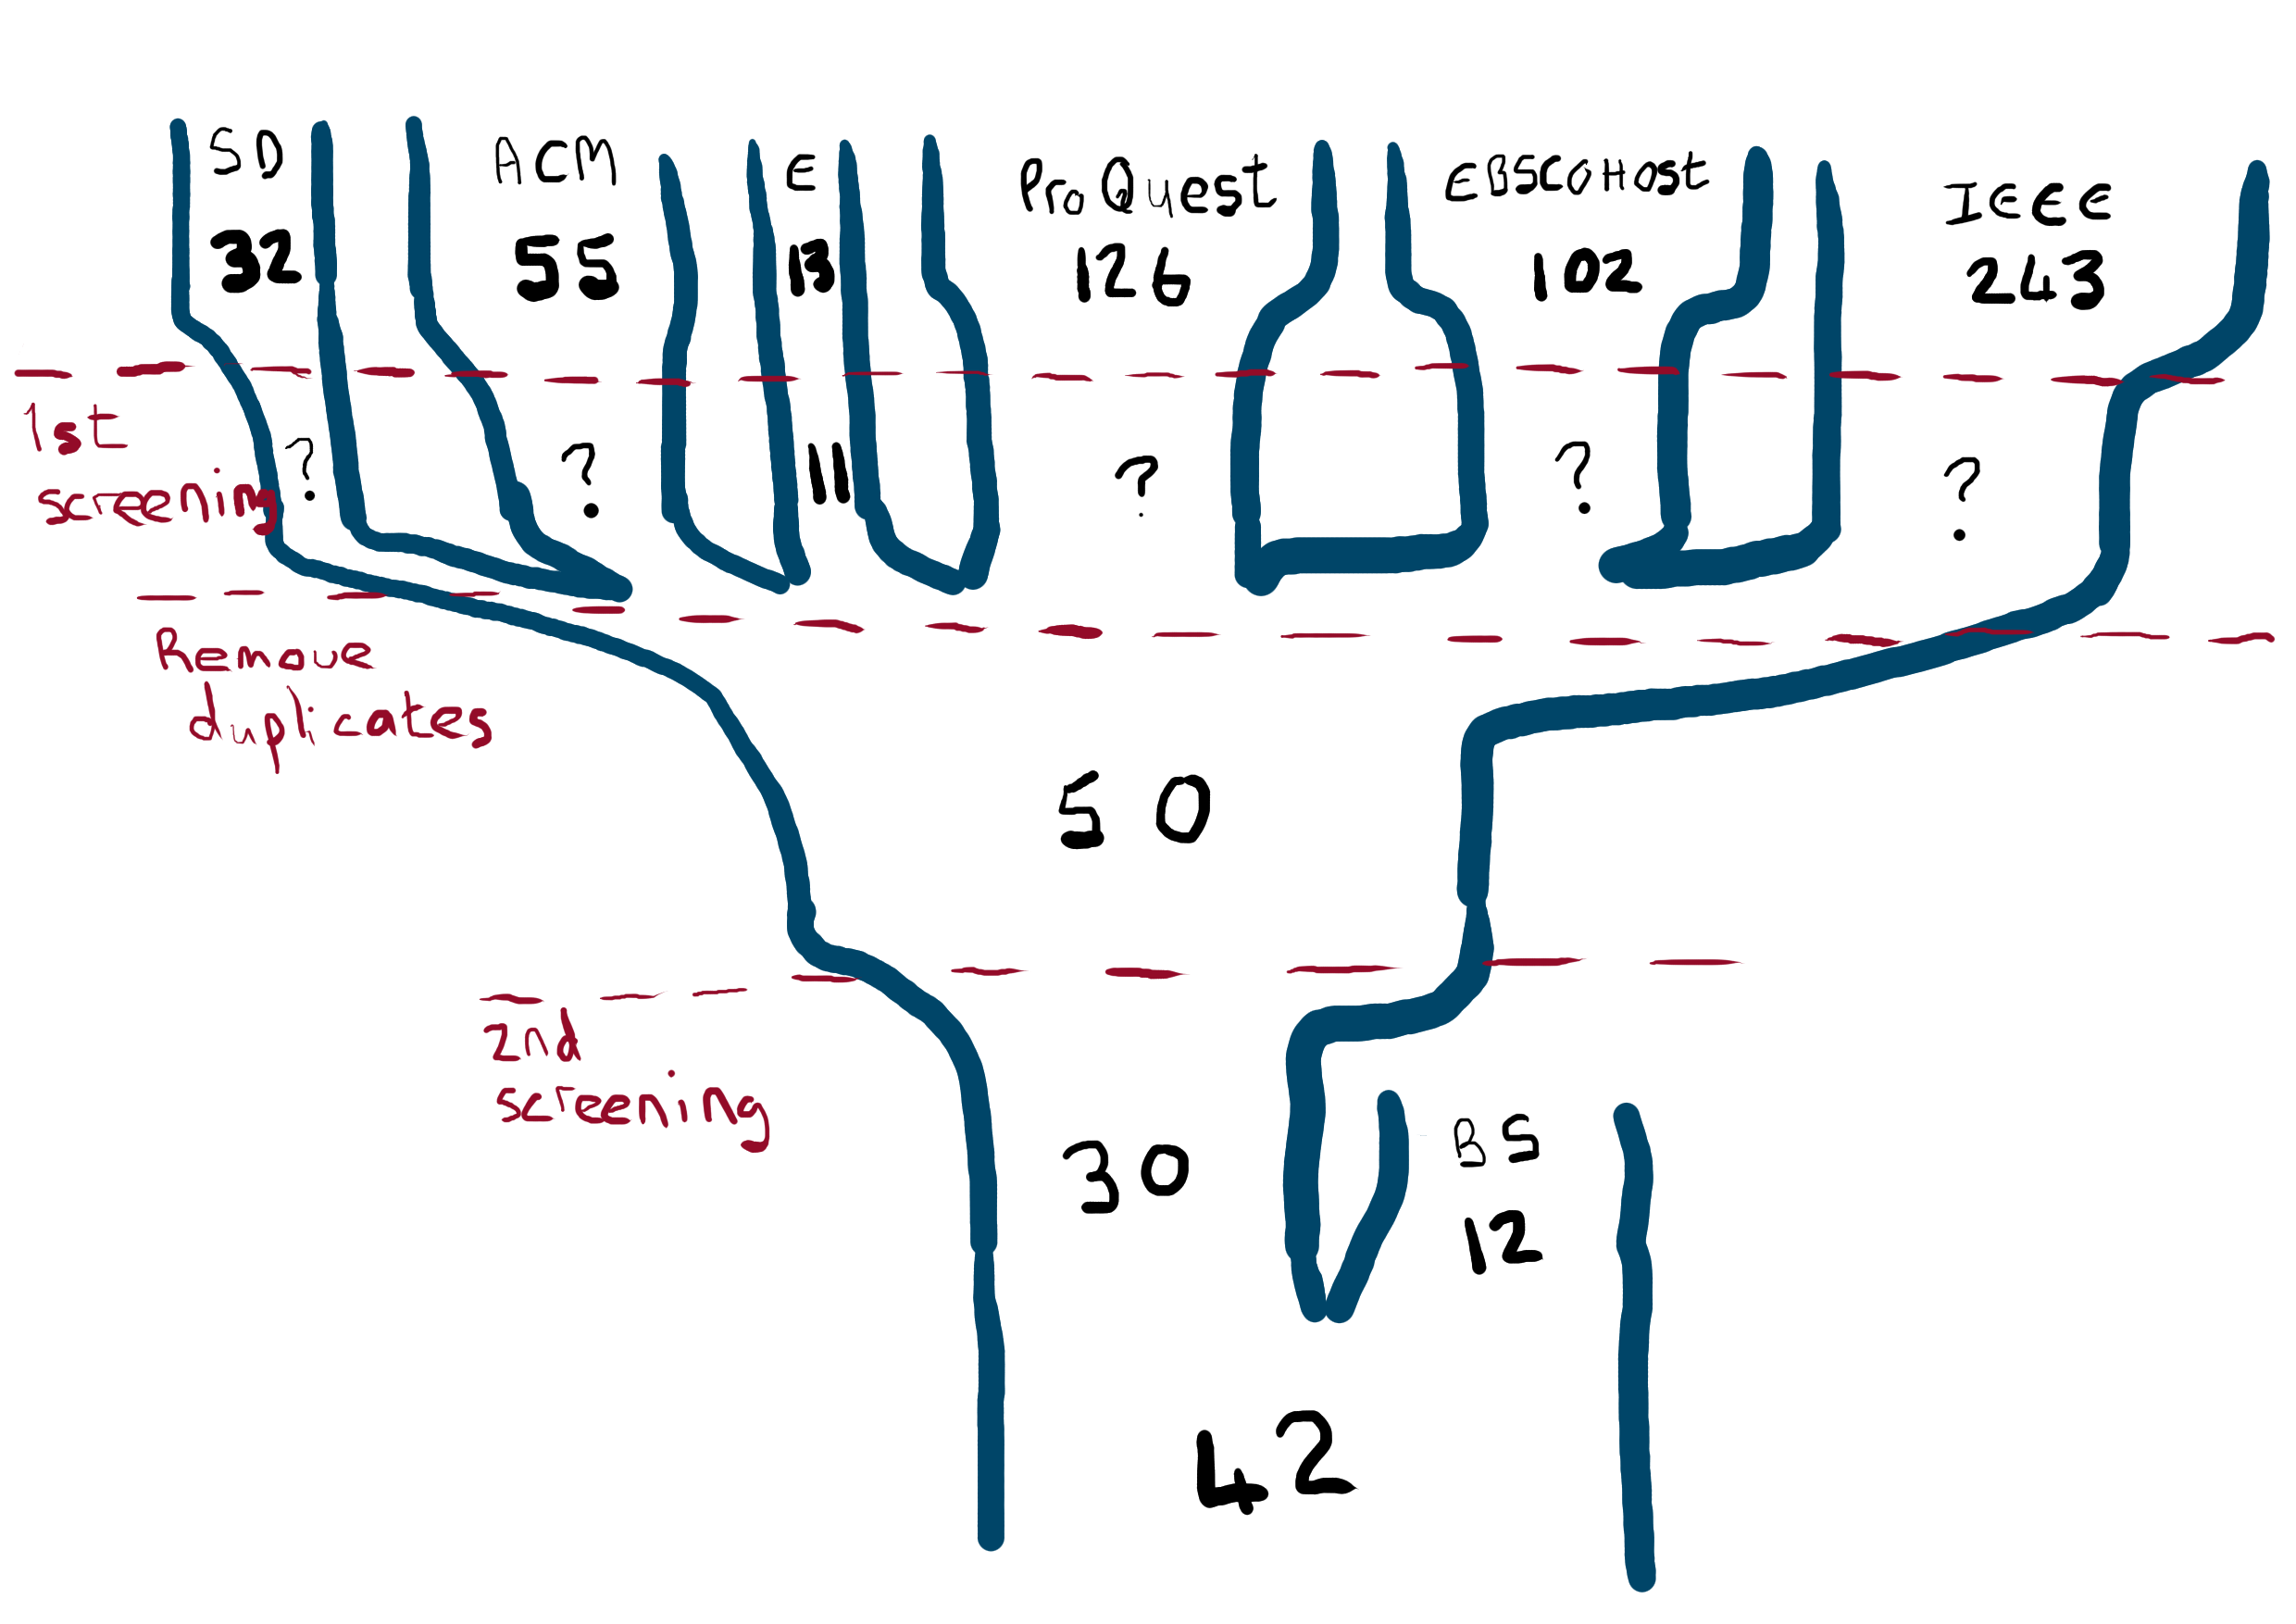
\includegraphics[width=\textwidth]{why_methodologies_exist/sankey}
\caption{Literature search and screening results}
\label{fig:search_lit}
\end{figure}

Springer was part of the search plan, but their search does not work with boolean operators when used in the title.
This resulted in Springer not forming part of the searched collections.

The combined results contained 543 \pieter{Why doesn't this add up? 🤔} items from 1972 to 2022 as the entire history was considered.
There was also no restriction on the sources of financial support for results.
However, the only restriction that did exist was articles had to be written in English.

\subsection{Screen for inclusion}
Two sets of screening was used to filter this list.
First, the results were evaulated on their abstracts and duplicates were removed which created a list of 50 results.
The criteria for inclusion at this step was for articles to explain ``why'' methodologies existed or were created.

\subsection{Assess quality}
The second set of screening involved downloading the full article for these 50 results and evaluating their abstract, introduction, and conclusion for further consideration.
It was not possible to get the full article for 6 of these results, and 1 result only had its title and abstract in English.
The remaining 43 results were evaluated and given a rank from 1 to 5.
A rank of 5 was given to the articles most relevant for ``why methodologies exist'' and a rank of 1 for least relevant.

Since this is a descriptive systematic literature review, the qualities in terms of references of each result was ignored to be able to built an accurate historic picture of ``why methodoligies exist''.
However, it was decided to analyse the results of all final rankings that were not deemed least relevant which reduces the final result to 30 items.

\subsection{Extract data}
Extracting data involved reading each result's full-text and trying to identify the reasons ``why a methodology existed''.
In most results, these reasons where in the form of bullet points where each bullet item was a reason answering the ``why''.
Each of these items were extracted to a list and linked back to the result it came from.

\subsection{Analyze and synthesize data}
This list was then grouped into ten year periods to understand how requirements changed with each era.
For each ten year period, the list items was accumulated together when the items were the same or had the same meaning.
This involved distilling similar reasons into one common phrase to be an umbrella term for all the items under it.
These umbrella terms were also kept consistent over each era.

\pieter{A backward search section is missing here}

\subsection{Report findings}
The finding for each era now follows. \pieter{the first methodology was documented in 1956 but this search first result is from the 1970s}

\subsubsection{1970s}
In this period software development is still new with many practices being borrowed from engineering.
It was, therefore, found that the structured methodologies of the time promised to improve programmer's productivity.
For the rest of this review, we will refer to improving productivity as resource management.
Methodologies also tried to improve the reliability, maintainability, and quality of the end product \cite{yourdon_1977}.

In this period personal computers made their entrance for the first time.
However, engineers still wrote most software to perform a specific task, for example flying Project Apollo\pieter{what are the physical aspects of project apollo}.
These systems would have clearly defined procedures written by engineers that the software would need to follow.
Hence, why quality and reliability was important in this period.

At the same time it would not be possible to update the program flying Apollo in mid-flight. \pieter{qualify}
Therefore, maintainability refers more to the short-term maintainability that would be needed before take-off.

In this period, methodologies were not a complete lifecycle encompassing package as they are today \cite{soi_1982, beregi_1985}.
Rather, there was a separate methodology for design (like structured design) and another methodology for implementation (like structured programming) and yet another for analysis (structured analysis).
Using them together was optional, thus it was possible to swap structured programming for top-down development while still using structured design. \cite{yourdon_1977}

\subsubsection{1980s}
In the early 1980s it was proposed that a methodology would be more successful if it covered all the development phases \cite{soi_1982}.
And by the mid 1980s, these phase based methodologies and the tools they used would start to be combined.
The term methodology was retained to describe this combination of phases and tools \cite{beregi_1985}. \pieter{See if there is a thausuris tool}

When looking at all the phases of development, cost became a concern to manage and reduce \cite{vanderlei_1983, peacham_1985, loesh_1985}.
Managing time became important as it had an impact on cost and timeliness ensures the system is not obsolete by the time it is operational because it took too long to be developed \cite{peacham_1985, beregi_1985, mannino_1987, paul_1993}.
This completes the triad of cost, time, and quality being important, but for any project, only two could be chosen.\pieter{where has quality gone}\pieter{can only take away if there is something else about quality}

Futher to cost, time, and quality, methodologies were used to manage:
\begin{itemize}
    \item User needs \cite{peacham_1985}
    \item Maintainability \cite{peacham_1985}
    \item Identifying the correct problem to solve which we will call risk \cite{peacham_1985}
    \item Proper documentation of the system \cite{loesh_1985}
    \item Cooperation between developers, users, and management and to establish jargon for their communications \cite{loesh_1985}
    \item Overall resource management \cite{mannino_1987}
\end{itemize}

\subsubsection{1990s}
By the start of the early 1990s, methodologies which integrate the entire development process were trending.\pieter{check be verbs}
While this is happening, software projects become smaller with end user applications rising in popularity.
This causes the overall perspective to be more focused on collecting the correct requirements \cite{paul_1993} from the end users.
For example, end user satisfaction made an appearance for why a methodology is needed.
\cite{drake_1991}

Overall the reasons for using methodologies in the 1990s were to:\pieter{time, cost and quality}
\begin{itemize}
    \item Minimize risk \cite{drake_1991, trussel_1999}
    \item Reduce cost \cite{drake_1991, scarre_1992, paul_1993}
    \item Timely delivery \cite{drake_1991, scarre_1992, herald_1993, trussel_1999}
    \item Resource management \cite{drake_1991}
    \item Team management \cite{drake_1991}
    \item Scheduling \cite{drake_1991, paul_1993}
    \item End user satisfaction \cite{drake_1991}
    \item Senior management awareness \cite{drake_1991}
    \item Quality \cite{drake_1991, scarre_1992, herald_1993, trussel_1999}
\end{itemize}

The definition for quality is, however, starting to make a shift towards non-functional requirements and the quality of the methodology's documentation \cite{scarre_1992}.
And the need to establish criteria to evaluate the final software in earlier phases is identified \cite{paul_1993, herald_1993, grossman_1997}.

\unsure{I think my tense shifted from past tense. Which tense should I be writing in? When talking about the past? future imperfect}

\subsubsection{2000s and beyond}
For the last 20 years many methodologies were created for specific non-functional requirements such as performance and security.
Therefore, these results will not be considered as reasons why methodologies exist since correctly identifying and managing this single requirement is part of minimizing risk.

There were still 3 articles though that listed the following reasons for using a methodology: \pieter{same grouping as earlier} \pieter{a diagram/visual.... in summary}
\begin{itemize}
    \item Team management \cite{lucena_2008}
    \item Control scope \cite{lucena_2008}
    \item Timely delivery \cite{lucena_2008, garg_2015}
    \item Cost \cite{lucena_2008, uzturk_2013, garg_2015}
    \item Managing changing or critical requirements \cite{lucena_2008, uzturk_2013}
    \item Risk management \cite{lucena_2008, uzturk_2013, garg_2015}
    \item Planning, scheduling and velocity measurements \cite{uzturk_2013}
    \item Common communication language \cite{uzturk_2013}
    \item Makes each role aware of their responsibility and what to do next \cite{uzturk_2013}
    \item Quality \cite{garg_2015}
\end{itemize}

\subsection{When a methodology is not used}\unsure{I don't know if this will be unneeded fluff... discuss first}
